\section{Neoplasie dell'osso}

Le neoplasie dell'osso e dei tessuti molli possono essere:

\begin{itemize}
\item
  \textbf{primitive}, cioè che iniziano e si sviluppano nel tessuto osteo-articolare
\item
  più frequentemente, \textbf{neoplasie secondarie} a metastasi, da tumori primitivi localizzati in altre regioni.
\end{itemize}

La patologia osteo-articolare primitiva tende ad interessare bambini ed adolescenti, anche per questo sono tumori molto aggressivi e resistenti alla terapia; per queste malattie è necessario un approccio multidisciplinare.

\subsection{Definizioni}

Alcune definizioni prima di trattare i tumori più frequenti:

\begin{itemize}
\item
  \textbf{IPERPLASIA:} accumulo di cellule dovuto o ad una proliferazione accelerata o ad una maturazione cellulare rallentata.
  Indotta da uno stimolo, scompare quando questo finisce. Solitamente il tessuto è costituito da una struttura cellulare ``organoide'' simile all'organo di origine.
\\
Alcuni esempi: callo osseo esuberante attorno ad un focolaio di frattura, miosite ossificante (calcificazione del tessuto muscolare, iperplastico) per stravaso ematico a seguito di uno strappo muscolare
importante.
\item
  \textbf{AMARTOMA:} tumore benigno che deriva da AMARTIA, cioè un'isola di tessuto che durante lo sviluppo embrionale, fetale o infantile viene esclusa dall'organizzazione regionale. Questa porzione di tessuto può continuare a crescere dopo la nascita costituendo un amartoma.
\\
Alcuni esempi: esostosi a livello della testa del perone, questo ``becco osseo'' viene rimosso per evitare la compressione del nervo sciatico;
origina da abbozzi cartilaginei fetali che possono accrescersi durante la vita extrauterina formando amartomi; angioma cutaneo (amartoma del tessuto vascolare).
\item
  \textbf{TUMORE BENIGNO:} neoformazione a crescita autonoma ma più lenta del maligno, non presenta atipie cellulari e organizzazione cellulare ``organoide'', con cellule ben differenziate. Si tratta di un tumore ben delimitato, che cresce per continuità, non causa metastasi e non recidiva dopo exeresi.
\\
Alcuni esempi: osteoma osteoide e tumore a cellule giganti.
\item
  \textbf{TUMORE MALIGNO:} può essere a basso, medio o alto grado a seconda dell'aggressività.
Si tratta sempre di neoformazioni a \emph{crescita autonoma}, con velocità di crescita \emph{elevata}, le cellule sono \emph{atipiche} e si organizzano in modo anarchico all'interno del tessuto di origine, poco differenziate, possono causare metastasi e, se non completamente asportate, possono recidivare localmente.
\\
Alcuni esempi: osteosarcoma, tumore maligno del tessuto osseo con prognosi altamente negativa; condrosarcoma, tumore maligno del tessuto cartilagineo.
\end{itemize}

Per classificare i tumori dell'osso primitivi è importante verificarne la \textbf{localizzazione}:

\begin{itemize}
\item
  \textbf{INTRACORTICALE:} crescita all'interno della corticale ossea
\item
  \textbf{INTRAMIDOLLARE:} crescita all'interno dell'osso spugnoso sottocorticale
\item
  \textbf{PERIOSTALE:} crescita sulla superficie esterna dell'osso a livello diafisario, dove è presente periostio
\item
  \textbf{PAROSTALE} O IUXTACORTICALE: crescita sulla superficie esterna dell'osso, nelle metafisi dove non ho periostio. Lo sviluppo è nel punto di inserzione di capsula articolare, tendini e legamenti
\end{itemize}

\subsection{Classificazione}

In base al tipo di tessuto prodotto dal tumore:

\begin{itemize}
\item tessuto osseo (neoplasie ossee osteoformative)
\item tessuto cartilagineo (neoplasie ossee condroformative)
\item tessuto vascolare
\item diversi tessuti molli (tessuto adiposo, fibroso, sinoviale)
\end{itemize}

In base alle caratteristiche istologiche (importante per terapia e prognosi), per definire il grado di malignità del tumore (basso, medio o alto), si valuta:

\begin{itemize}
\item cellularità
\item atipie
\item differenziazione
\item encapsulazione (fattore prognostico positivo)
\end{itemize}

In base al tipo di cellule che compongono il tumore e al tessuto da cui derivano:

\begin{itemize}
\item fibroblasti e tessuto fibroso (fibroma, benigno, o fibrosarcoma, maligno)
\item condroblasti o tessuto cartilagineo (condroma o -sarcoma)
\item osteoblasti o tessuto osteoide (osteoma o -sarcoma)
\end{itemize}

Per curare le neoplasie ossee esistono dei centri regionali, il nostro centro di riferimento è l'Istituto Rizzoli di Bologna.

\subsection{Diagnosi}

In caso di sospetto di neoplasia ossea, la diagnosi si basa su clinica, esami strumentali e conferma bioptica. In alcuni casi, come osteoma osteoide del calcagno, si ha certezza della diagnosi solo attraverso gli esami strumentali, poiché questo tumore presenta caratteristiche radiografiche preminenti.

In generale la diagnosi si basa su:

\subsubsection{Anamnesi e caratteristiche cliniche del paziente}

\begin{itemize}
\item \textbf{età:}
\begin{itemize}
\item tumore a cellule giganti: raro prima della pubertà
\item sarcoma di Ewing (si localizza soprattutto a livello del ginocchio): raro prima dei 5 anni e dopo i 30
\item condrosarcoma: raro nel bambino
\end{itemize}
\item \textbf{velocità di accrescimento:} rapida nei tessuti maligni
\item \textbf{iperpiressia:} indicativa di \emph{sarcoma di Ewing}
\item \textbf{dolore:}
\begin{itemize}
\item tipicità di alcuni tumori (osteoma osteoide causa un dolore tipicamente notturno)
\item dolore da \emph{frattura patologica} (improvviso ed acuto)
\item il \emph{condrosarcoma} è più doloroso del condroma
\item il \emph{sinovial sarcoma} è estremamente doloroso
\end{itemize}
\item \textbf{localizzazione:} 
\begin{itemize}
\item il \emph{condroma} è tipico nella mano a livello delle falangi
\item il \emph{tumore a cellule giganti} si localizza prevalentemente a livello delle metaepifisi delle ossa lunghe
\end{itemize}
\end{itemize}

\subsubsection{Radiografia (deve sempre essere eseguita)}

Ci permette di vedere:

\begin{itemize}
\item
  \textbf{OSTEOLISI}, di cui si valuta:
\begin{itemize}
\item
  \emph{velocità di crescita}
\item
  Intaccamento delle corticali
\item
  presenza di osteogenesi reattiva
\item
  presenza di orletto sclerotico (osteoma osteoide).
\end{itemize}
\item \textbf{OSTEOGENESI REATTIVA}
\item \textbf{ESPANSIONE DEI TESSUTI MOLLI}
\item \textbf{CALCIFICAZIONI NEI TESSUTI MOLLI}
\end{itemize}

\subsubsection{Angiografia}

Permette di valutare:

\begin{itemize}
\item
  la presenza di vascolarizzazione nel tumore (criterio prognostico negativo)
\item
  i rapporti con i vasi (importante prima dell'intervento valutare se un grosso vaso è stato intaccato o compresso)
\item
  i margini tumorali nei tre piani spaziali.
\end{itemize}

\subsubsection{Scintigrafia con Tc 99}

Permette di:

\begin{itemize}
\item
  valutare se la neoplasia è captante il Tecnezio
\item
  visualizzare tutto lo scheletro e le neoformazioni non visibili all'Rx o localizzate a distanza (metastasi)
\item
  è un indice di \emph{quiescenza o} di \emph{attività} del tumore.
\item
  Rappresenta uno strumento utile nel post-operatorio per visualizzare possibili \emph{recidive} e anche nella valutazione della \emph{risposta} a radio e chemioterapia.
\end{itemize}

\subsubsection{TAC}

Utile per valutare l'\textbf{estensione} del tumore e i
\textbf{rapporti} con vasi,visceri e strutture vascolari circostanti.

\subsubsection{RMN}

Strumento utile per lo studio dei \textbf{tessuti molli} e del \textbf{tessuto adiposo}, soprattutto dopo somministrazione di mezzo di contrasto che ne aumenta la sensibilità.

\subsubsection{Biopsia}

Fondamentale per \textbf{completare la diagnosi}.

Bisogna però considerare che si tratta di un compromesso fra il desiderio di \emph{ottenere tessuto} per una diagnosi certa e il \emph{rischio di spargere} inopportunamente \emph{cellule neoplastiche} che potrebbero complicare la terapia.

Per ridurre il rischio di diffusione delle cellule neoplastiche, la via di accesso di una biopsia incisionale dovrebbe essere localizzata lungo la linea di incisione del trattamento chirurgico definitivo.

Esistono diverse tipologie di biopsia:

\begin{itemize}
\item
  \textbf{\emph{AGOBIOPSIA}:} aspirazione di poche cellule, con scarso rischio di contaminazione neoplastica, possibile solo per \emph{tumori molli} senza capsula ossea, ma a causa della scarsa raccolta può avere un'alta incidenza di falsi negativi.
\item
  \textbf{\emph{BIOPSIA CON TROCAR}} (aghi di dimensioni maggiori e cannulati)\textbf{:}utilizzata per i \emph{tessuti ossei}, si raccolgono ``losanghe'' di tessuto di 3- e, per questo motivo, vi è un maggiore rischio di contaminazione neoplastica ma al tempo stesso una minore incidenza di falsi negativi.
\item
  \textbf{\emph{BIOPSIA INCISIONALE}:} eseguita se le precedenti non hanno dato risultati certi e nei casi in cui sia richiesto molto tessuto.
\end{itemize}

\subsection{Trattamento}

Può essere di tre tipi:

\begin{itemize}
\item[1.]
  \textbf{ASTENSIONISTICO:} valuto nel tempo come evolvono certi tumori benigni o pseudo tumori, che possono anche autolimitarsi nel tempo
\item[2.]
  \textbf{CHIRURGICO} con o senza adiuvanti (fenolo,alcol), utilizzati per distruggere le cellule tumorali, ed innesti ossei: si può eseguire un'escissione più o meno ampia
\item[3.]
  \textbf{CHEMIO} o \textbf{RADIOTERAPIA:}
\begin{itemize}
\item
  \emph{neoadiuvanti}, ovvero prima del trattamento chirurgico. Permettono la riduzione delle dimensioni della massa tumorale.
\item
  \emph{adiuvanti}, cioè post-intervento. Per rimuovere le cellule neoplastiche rimaste.
\end{itemize}
\end{itemize}

\subsubsection{Trattamento chirurgico}

L'\textbf{escissione} può essere più o meno ampia a seconda della localizzazione dei margini chirurgici, cioè dalla quantità e qualità dei tessuti che ricoprono il tumore dopo la sua asportazione.

Esistono varie tipologie di asportazione:

\begin{itemize}
\item
  \textbf{INTRALESIONALE}, quando il tumore è ``sbucciato'' della sua capsula o pseudo capsula (quindi viene enucleato) o interrotto anche in una minima area della sua superficie; per il rischio di lasciare cellule tumorali in situ viene utilizzata solo per \emph{neoplasie a bassa malignità} (osteoma osteoide, tumore a cellule giganti, cisti ossee) e si fa uso di adiuvanti come fenolo o alcol durante l'intervento.
All'interno delle cisti viene addirittura inserito cemento.
\item
  \textbf{MARGINALE}, quando il tumore viene rimosso in blocco completamente ricoperto dalla sua capsula o pseudo capsula
\item
  \textbf{AMPIA}, quando il tumore è rimosso in blocco e completamente ricoperto da uno strato continuo di tessuto normale
\item
  \textbf{RADICALE}, quando il tumore è rimosso in blocco con l'intero compartimento anatomico di origine circondato dalle sue naturali barriere (ad esempio se si rimuove il femore in toto).
\end{itemize}

\subsection{Tumori benigni osteoformatori}

\subsubsection{OSTEOMA OSTEOIDE}

Si tratta di una piccola e dolente neoformazione costituita da \textbf{tessuto osteoide}, osso intrecciato, e circondato da un piccolo e dolente \emph{alone reattivo}, cioè un orletto sclerotico reattivo attorno alla lesione.

\paragraph{Epidemiologia}
Colpisce i giovani fra i 5 e i 30 anni, con un rapporto M/F 2,5/1

\paragraph{Localizzazione}
Di solito colpisce la zona diafiso-metafisaria corticale dello scheletro appendicolare

\paragraph{Clinica}
Si tratta di un tumore molto vascolarizzato che causa dolore notturno sensibile all'acido acetilsalicilico, perché è un tumore che produce al suo interno un'ingente quantità di prostaglandine e il farmaco va a bloccare questa produzione.

\paragraph{Diagnosi strumentale}
L'osteoma osteoide è visibile alla radiografia con due segni specifici, cioè la presenza di un'osteolisi a ``nidus'' e attorno ad essa la presenza di un orletto sclerotico.
La scintigrafia ossea è positiva con un quadro di ``faro nella nebbia''
Un'ulteriore indagine può essere rappresentata dalla TAC con m.d.c.

\paragraph{Trattamento}
Asportazione chirurgica della neoformazione
Il tessuto patologico ha un aspetto molto diverso rispetto all'osso normale, che è giallastro, perché si presenta di colore rossastro dovuto all'ingente vascolarizzazione.

Nelle localizzazioni molto profonde come a livello del collo femorale o a livello vertebrale si possono eseguire degli interventi di radiologia interventistica, che vanno a distruggere l'osteoma osteoide con le radiofrequenze.

\begin{figure}[!ht]
\centering
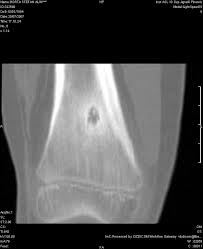
\includegraphics[width=0.4\textwidth]{010/image1.jpeg}
\end{figure}

In questa immagine radiologica si può notare il tipico aspetto a ``nidus'' dell'osteoma osteoide con la parte biancastra attorno che rappresenta l'orletto sclerotico.

\subsection{Tumori maligni osteoformatori}

\subsubsection{OSTEOSARCOMA}

Tumore maligno costituito da \textbf{cellule mesenchimali} che producono tessuto osteoide e \textbf{osseo immaturo}.

\paragraph{Epidemiologia}
Colpisce i giovani, generalmente fra i 10 e i 20 anni; M/F 2/1; si tratta del secondo tumore osseo maligno per frequenza dopo il condrosarcoma

\paragraph{Localizzazione}
A livello diafiso-metafisario delle ossa lunghe (70\% ginocchio e spalla)

\paragraph{Clinica}
Compare dolore e ci può essere una tumefazione calda, limitazione del movimento articolare e febbre. Essendo un tumore che determina osteolisi, vi sarà un aumento tipico di fosfatasi alcalina e LDH.

\paragraph{Diagnosi strumentale}
Dal punto di vista radiologico si vede un'evoluzione della lesione: il tumore inizialmente è intraosseo, poi tende a diventare extraosseo.
La scintigrafia ossea è positiva, come TAC e RMN.
Caratteristiche radiologiche peculiari: osteolisi ed addensamenti con reazione periostale ``a sole nascente''

\begin{figure}[!ht]
\centering
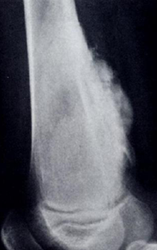
\includegraphics[width=0.4\textwidth]{010/image2.png}
\end{figure}

\paragraph{Trattamento}
Solitamente il trattamento è \textbf{doppio}:
\begin{itemize}
\item[1.]
  \emph{chemioterapia pre-operatoria}, 2 mesi prima dell'asportazione, per ridurre le dimensioni del tumore
\item[2.]
  \emph{escissione radicale} della neoplasia.
\end{itemize}
A seguito dell'asportazione possono essere posizionate delle \textbf{protesi tumorali specifiche} (ad esempio a livello del ginocchio), molto spesso fatte su misura per il paziente, che vanno a sostituire gran parte o totalmente femore e tibia.
